
\documentclass[onecolumn]{article}
\usepackage{graphicx}

\begin{document}
\title{\Large\bf Odin OS scheduler interface and implementation}
\author{Stanislav Karchebny, \\
        email: \texttt{berk@madfire.net}}
\maketitle



\section{Introduction}
\label{sec-intro}

\par This document describes implementation of scheduler component for Odin OS \cite{odin}.
The scheduler is primarily used to achieve a level of "multitasking" for system and user processes.
This scheduler exploits thread priorities when "scheduling" execution, allowing high-priority and
low-priority threads. It also mimics a feature of modern operating systems like Windows NT \cite{winnt}
and some Unices as dynamic-priority and fixed-priority threads.



\section{Threads}
\label{sec-threads}

\par In a multitasking system there can be alot of
programs, also called \emph{"processes"} from the operating system point of view, that consist of one or
more \emph{threads}. Threads are the minimal indivisible entities of program execution. Their life cycle
is depicted on Figure \ref{fig:life-cycle}.

\begin{center}
\begin{figure}[ht]
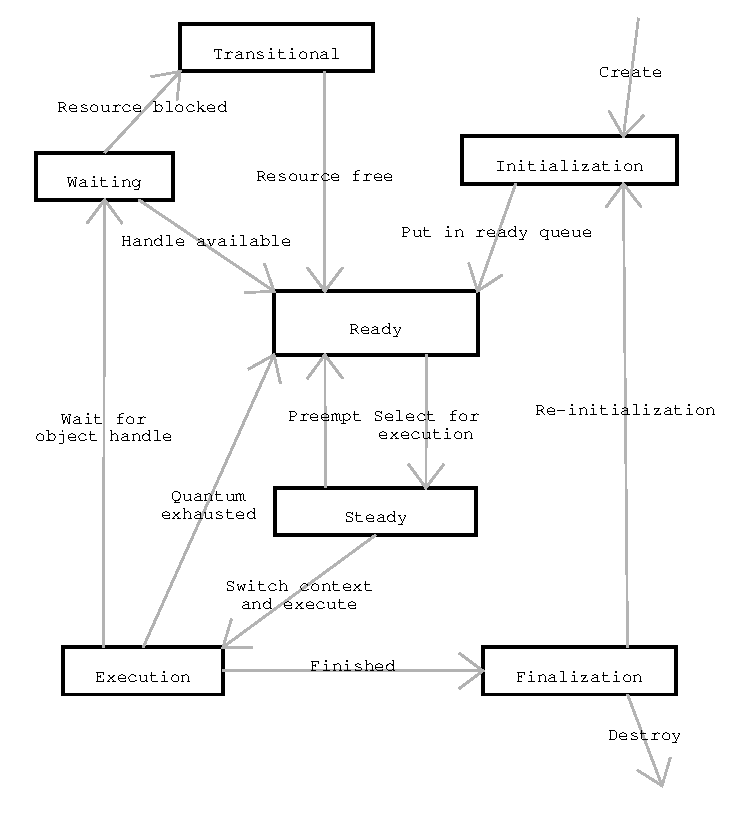
\includegraphics{process_life_cycle.eps}
\caption{Thread life-cycle graph}
\label{fig:life-cycle}
\end{figure}
\end{center}


\subsection{Thread interface}
\label{sec-thread-interface}

\par Odin thread is represented via its \emph{interface}:

\small
\begin{verbatim}
interface thread
{
   void ctor();           // constructor
   void dtor();           // destructor

   void run();            // thread's payload - execution method

   // ??
   void sleep(void);      // put current thread into sleep
   void yield(void);      // run the most appropriate thread
};
\end{verbatim}
\normalsize



\section{Scheduler}
\label{sec-sched}

\par The scheduler itself.


\subsection{Scheduler interface}
\label{sec-sched-interface}

\par The scheduler interface.

\small
\begin{verbatim}
interface sched
{
   void ctor();           // constructor
   void dtor();           // destructor

   void sleep(void);      // put current thread into sleep
   void sleep(thread t);  // put t into sleep
   void wake(thread t);   // wake up t
   void yield(void);      // run the most appropriate thread
};
\end{verbatim}
\normalsize


\subsection{Scheduler thread dispatching policy}
\label{sec-sched-dispatch}

\par The scheduler dispatching policy determines how threads priorities are treated and how existing
and newly created threads are scheduled.

\begin{figure}[ht]
\begin{center}
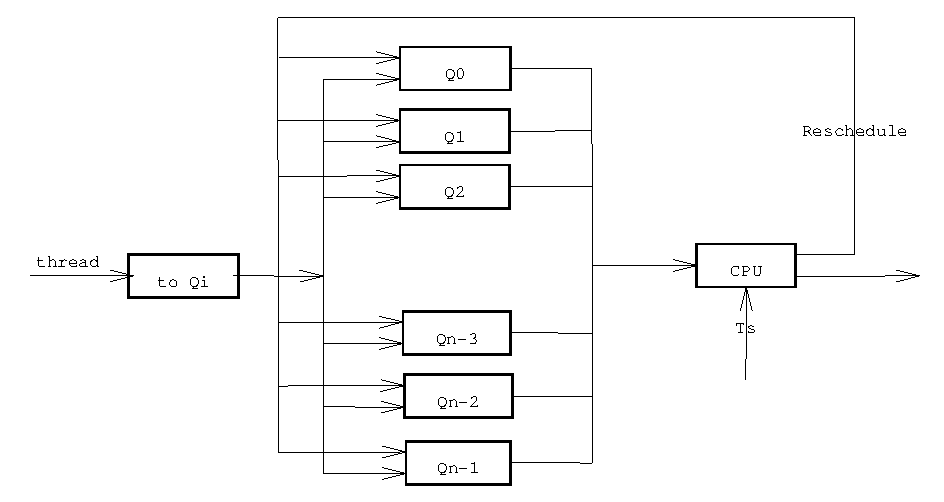
\includegraphics{PMQT.eps}
\caption{Dispatching via PMQT}
\label{fig:dispatch-pmqt}
\end{center}

\par Designations
\begin{description}
\item[ thread ] incoming new scheduled thread
\item[ Ts ] service time quantum
\item[ Tr ] service time taken by thread
\end{description}

\par Rescheduling is done as follows:
\begin{enumerate}
\item if 0 <= i < R then to Qi
\item else if preempted then to Qi
\item      else if Tr >= Ts then to Qi+1
\item      else (Tr < Ts) to Qi-1
\end{enumerate}

\end{figure}

\par As per POSIX standard \cite{posix}, sched::select() always selects thread from head of the most
prioritive queue.

\small

\bibliographystyle{plain}
\bibliography{odin}

\end{document}
